%% SPECIFICA TECNICA

%controllare gli svantaggi

\section{Introduzione}
\subsection{Scopo del documento}

Questo documento ha come scopo quello di definire la progettazione ad alto livello
per il prodotto Monolith. Verrà presentata l’architettura generale secondo la quale
saranno organizzate le varie componenti software e i Design Pattern utilizzati nella
creazione dell'SDK, delle bolle predefinite e della demo. Verrà inoltre dettagliato il tracciamento tra le componenti software individuate ed i requisiti.


\subsection{Scopo del prodotto}

Lo scopo del prodotto è quello di permettere la creazione di bolle
interattive, che dovranno funzionare nell’ambiente Rocket.chat. Queste
bolle permetteranno di aumentare l'interattività tra gli utenti della
chat e aggiungeranno nuove funzionalità accessibili direttamente dalla conversazione 
senza il bisogno di ricorrere all'apertura di applicazioni diverse.
Il sistema offrirà agli sviluppatori un set di \glossario{API} per creare e
rilasciare nuove bolle e agli utenti finali la possibilità di
usufruire di un insieme di bolle predefinite.


\subsection{Glossario}

Al fine di evitare ogni ambiguità di linguaggio e massimizzare la
comprensione dei documenti, i termini che necessitano di essere
chiariti saranno scritti in corsivo e marcati con una |G| in pedice alla prima
occorrenza e saranno riportati nel Glossario.

\subsection{Riferimenti}

\subsubsection{Normativi}
\begin{itemize}
	\item \textbf{Norme di Progetto}: \\ NormediProgetto\_v1.1.0
	\item \textbf{Capitolato d'appalto C5}: \\ \url{http://www.math.unipd.it/~tullio/IS-1/2016/Progetto/C5.pdf}
	\item \textbf{Analisi dei Requisiti}: \\ AnalisideiRequisiti\_v1.0.0
	
\end{itemize}


\subsubsection{Informativi}
\begin{itemize}
	\item \textbf{Slide del corso di Ingegneria del Software}: \\  \url{http://www.math.unipd.it/~tullio/IS-1/2016/ }
\end{itemize}

\section{Tecnologie Utilizzate}

In questa sezione verranno descritte le tecnologie su cui si basa lo sviluppo del progetto. Per ognuna di esse, verranno indicati l’ambito di utilizzo della tecnologia, i vantaggi e gli svantaggi che ne derivano.Alcune delle tecnologie che saranno usate sono richieste come requisito dal capitolato scelto.

\subsection{Javascript 6th edition (ECMA SCRIPT 6)}

JavaScript è un linguaggio di scripting orientato agli oggetti e agli eventi. \'E comunemente utilizzato nella programmazione Web lato client per la creazione, in siti web e applicazioni web, di effetti dinamici interattivi tramite l'uso di funzioni di script invocate da eventi innescati in vari modi dall'utente sulla pagina web in uso. \\ Come richiesto dal capitolato, per la realizzazione di Monolith, deve essere utilizzato Javascript 6th edition (ECMA SCRIPT 6). \\

\textbf{Licenza}:  \\
Non esiste una sola implementazione perché ECMAScript (o ES) è un linguaggio di programmazione standardizzato e mantenuto da Ecma International nell'ECMA-262 ed ISO/IEC 16262.


\textbf{Vantaggi}: 
\begin{itemize}
	\item Gestione degli eventi asincroni tramite le promises
	\item Possibilità di dichiarare classi
	\item Supporto per le costanti(\emph{const})
	\item Possibilità di isolare la definizione di variabili ad un blocco (\emph{let})
	\item Possibilità di isolare lo scope di una funzione usando blocchi delimitati da parentesi graffe({}) come ambienti isolati (vs closure)
	\item Uso di sintassi più espressiva per scrivere le funzioni anonime (\emph{Arrow Functions})
	
\end{itemize}

\textbf{Svantaggi}: 
\begin{itemize}
	\item Il supporto di ES6 da parte dei browser è ancora incompleto
	\item L’assenza di tipizzazione potrebbe ostacolare la valutazione della correttezza del codice
\end{itemize}

\subsection{Meteor}

Meteor è un framework web JavaScript libero e open source  per lo sviluppo di applicazioni web e mobile. \'E una piattaforma basata su Node.js. Meteor utilizza, dunque, JavaScript sia lato client che lato server. 

\textbf{Licenza}: MIT \\
La licenza MIT è una delle licenze più permissive nel panorama open source. In modo più esplicito dichiara i diritti dati all'utente finale, incluso il diritto di utilizzare , copiare, modificare, incorporare, pubblicare, distribuire, sotto-licenziare, e/o vendere il software.


\textbf{Vantaggi}: 
\begin{itemize}
	\item Integrazione con diverse tecnologie utilizzate nello sviluppo web:
	\begin{itemize}
		\item React
		\item MongoDB
	\end{itemize}
	\item Isomorfismo: il codice javascript scritto funziona in modo trasparente sul client (browser), sul server (Node.js) o in entrambi i mondi
	\item Ecosistema e modularità: la comunità di Meteor è molto attiva e molte funzionalità client o server potrebbero già essere pacchettizzate dal package manager ufficiale. 
\end{itemize}

\textbf{Svantaggi}: %controllareeeeeee 
\begin{itemize}
	\item Inizialmente sconosciuto ai membri del gruppo.
	%\item Il modo in cui alcuni componenti core della tecnologia si interfacciano potrebbe limitare la libertà degli sviluppatori.
\end{itemize}

\subsection{Mongo DB}
MongoDB è un database NoSQL orientato ai documenti, basato sul formato JSON per la memorizzazione e la rappresentazione dei dati. \'E distribuito come software libero open source. \\

\textbf{Licenza}: GNU AGPL v3.0 \\
\'E una licenza pubblicata da Free Software Foundation. \'E simile alla capostipite GNU GPL, una licenza fortemente copyleft per software libero.

\textbf{Vantaggi}: 
\begin{itemize}
	\item \'E più flessibile di un database SQL e facilita la rappresentazione su un modello ad
	oggetti
	\item Supporta ricerche per campi, intervalli e regular expression. Le query possono restituire campi specifici del documento e anche includere funzioni definite dall'utente in JavaScript.
	\item Qualunque campo in MongoDB può essere indicizzato 
\end{itemize}


\textbf{Svantaggi}: 
\begin{itemize}
	\item Inizialmente sconosciuto ai membri del gruppo.	
\end{itemize}

\subsection{HTML5}
HTML5 è un linguaggio di markup per la strutturazione delle pagine web.

\textbf{Licenza}:  \\
Non esiste una sola implementazione perché HTML5 è un linguaggio di markup standardizzato e mantenuto da W3C.


\textbf{Vantaggi}: 
\begin{itemize}
	\item Codice più pulito e sintassi semplificata rispetto alle versioni precedenti
	\item Interattività senza l’ausilio di plugin esterni valida per diversi formati multimediali
	\item Semantica intuitiva grazie ai nuovi TAG di formattazione
	\item Introduzione della geolocalizzazione, dovuta ad una forte espansione di sistemi operativi mobili
	\item Sistema più efficiente alternativo ai normali cookie chiamato Web Storage 

\end{itemize}

\textbf{Svantaggi}: 
\begin{itemize}
	\item Non tutti i browser supportano HTML5
\end{itemize}

\subsection{SCSS}

SCSS è una sintassi per i fogli di stile introdotta da Sass 3 (Syntactically Awesome StyleSheets). \'E un'estensione del CSS .

\textbf{Licenza}: MIT \\
La licenza MIT è una delle licenze più permissive nel panorama open source. In modo più esplicito dichiara i diritti dati all'utente finale, incluso il diritto di utilizzare , copiare, modificare, incorporare, pubblicare, distribuire, sotto-licenziare, e/o vendere il software.

\textbf{Vantaggi}: 
\begin{itemize}
	\item Possibilità di utilizzare variabili
	\item Possibilità di creare funzioni 
	\item Possibilità di organizzare il foglio di stile in più file
	\item Compatibilità completa con la sintassi del CSS
\end{itemize}

\textbf{Svantaggi}: 
\begin{itemize}
	\item  Sintassi più complessa.
\end{itemize}

\subsection{React}

React è una libreria Javascript open source che permette di costruire interfacce utente. 

\textbf{Licenza}: BSD-3-Clause \\
Le licenze BSD sono una famiglia di licenze permissive, senza copyleft, per software.
Le tre clausole della licenza BSD-3-Clause sono:

\begin{itemize}
	\item Libertà di eseguire il programma per qualsiasi scopo
	\item Libertà di studiare il programma e modificarlo
	\item Libertà di ridistribuire copie del programma in modo da aiutare il prossimo
	
\end{itemize}

\textbf{Vantaggi}: 
\begin{itemize}
	\item Semplificazione della realizzazione di interfacce UI dinamiche che possono reagire ai cambiamenti di dati in maniera autonoma attraverso opportuni componenti
	\item Possibilità di utilizzare le viste per creare codice più facile da comprendere e su cui è più semplice effettuare il debugging.
	
\end{itemize}

\textbf{Svantaggi}: 
\begin{itemize}
	\item Implementa solo il livello view è quindi necessario utilizzare altre librerie per implementare altre parti dell'applicazione
	\item Curva di apprendimento ripida
	\item \'E una libreria relativamente nuova
\end{itemize}

\subsection{Node.js}

Node.js è una piattaforma event-driven per il motore JavaScript V8. Essa permette di realizzare applicazioni web utilizzando il linguaggio JavaScript, tipicamente client-side, per la scrittura anche della parte server-side.

\textbf{Licenza}: MIT \\
La licenza MIT è una delle licenze più permissive nel panorama open source. In modo più esplicito dichiara i diritti dati all'utente finale, incluso il diritto di utilizzare , copiare, modificare, incorporare, pubblicare, distribuire, sotto-licenziare, e/o vendere il software.

\textbf{Vantaggi}: 
\begin{itemize}
	\item Facile apprendimento
	\item Possibilità di realizzare applicazioni server-side senza dover imparare linguaggi di programmazione “tradizionali”
\end{itemize}

\textbf{Svantaggi}: 
\begin{itemize}
	\item Non supporta database relazionali
	
\end{itemize}

\subsection{Rochet.chat}

Rocket.chat è una Web chat server sviluppata in Javascript utilizzando il \glossario{Framework} Meteor.

\textbf{Licenza}: MIT \\
La licenza MIT è una delle licenze più permissive nel panorama open source. In modo più esplicito dichiara i diritti dati all'utente finale, incluso il diritto di utilizzare , copiare, modificare, incorporare, pubblicare, distribuire, sotto-licenziare, e/o vendere il software.

\textbf{Vantaggi}: 
\begin{itemize}

	\item Codice open source
	\item Possibilità di creare chat di gruppo
	\item Possibilità di inviare audio, video e file
	\item Possibilità di effettuare video chiamate
	\item Community molto attiva

	
\end{itemize}

\textbf{Svantaggi}: 
\begin{itemize}
	\item Parzialmente documentata
\end{itemize}

\subsection{Bootstrap}

Bootstrap è una raccolta di strumenti liberi per la creazione di siti e applicazioni per il Web. Essa contiene modelli di progettazione basati su HTML e CSS, sia per la tipografia, che per le varie componenti dell'interfaccia, come moduli, pulsanti e navigazione, così come alcune estensioni opzionali di JavaScript.

\textbf{Licenza}: MIT \\
La licenza MIT è una delle licenze più permissive nel panorama open source. In modo più esplicito dichiara i diritti dati all'utente finale, incluso il diritto di utilizzare , copiare, modificare, incorporare, pubblicare, distribuire, sotto-licenziare, e/o vendere il software.

\textbf{Vantaggi}: 
\begin{itemize}
	
	\item Piattaforma ben standardizzata 
	\item Non richiede l’appoggio né di un linguaggio di programmazione server side, né di un database
	\item Ottima documentazione
	\item Responsive Design	
	\item \'E supportato dai browser moderni
	
\end{itemize}

\textbf{Svantaggi}: 
\begin{itemize}
	\item I plugin di jQuery sono limitati
	\item Le modifiche dovute al continuo sviluppo non sono sempre facili da integrare
\end{itemize}



\subsection{polyglot.js}
Polyglot.js è una libreria per la traduzione scritta in JavaScript, eseguita sia per il browser che per gli ambienti CommonJS(Node).

\textbf{Licenza}: MIT \\
La licenza MIT è una delle licenze più permissive nel panorama open source. In modo più esplicito dichiara i diritti dati all'utente finale, incluso il diritto di utilizzare , copiare, modificare, incorporare, pubblicare, distribuire, sotto-licenziare, e/o vendere il software.

\textbf{Vantaggi}: 
\begin{itemize}
	\item Non è rischiesta una iscrizione per l'utilizzo
	\item \'E una libreria non a pagamento
	\item Il Polyglot ha zero dipendenze
	\item Copre una traduzione di 30 lingue diverse
\end{itemize}




\subsection{Money.js}

Money.js è una libreria semplice con l'unico obiettivo di convertire un valore di denaro da qualsiasi valuta in qualsiasi altra valuta. Money.js utilizza una fusione algoritmica per calcolare un insieme di tassi costantemente preciso per 165 valute mondiali. 

\textbf{Licenza}: MIT \\
La licenza MIT è una delle licenze più permissive nel panorama open source. In modo più esplicito dichiara i diritti dati all'utente finale, incluso il diritto di utilizzare , copiare, modificare, incorporare, pubblicare, distribuire, sotto-licenziare, e/o vendere il software.

\textbf{Vantaggi}: 
\begin{itemize}
	\item Non è rischiesta una iscrizione per l'utilizzo
	\item \'E una libreria non a pagamento
	\item \'E una libreria semplice da integrare nel codice JavaScript
\end{itemize}


\subsection{weather.js}

Weather.js è una libreria che recupera i dati da openweathermap.org e fa la ricerca di tutti i tipi di informazioni relative alle condizioni meteo.

\textbf{Licenza}: MIT \\
La licenza MIT è una delle licenze più permissive nel panorama open source. In modo più esplicito dichiara i diritti dati all'utente finale, incluso il diritto di utilizzare , copiare, modificare, incorporare, pubblicare, distribuire, sotto-licenziare, e/o vendere il software.

\textbf{Vantaggi}: 
\begin{itemize}
	\item Non è rischiesta una iscrizione per l'utilizzo
	\item \'E una libreria non a pagamento
	\item \'E una libreria semplice da integrare nel codice JavaScript
\end{itemize}

\textbf{Svantaggi}: 
\begin{itemize}
	\item Ha bisogno di 11 dipendenze 
\end{itemize}


\subsection{classNames}

classNames è una semplice utility raccomandata per l'uso con React per l'unione condizionata di className

\textbf{Licenza}: MIT \\
La licenza MIT è una delle licenze più permissive nel panorama open source. In modo più esplicito dichiara i diritti dati all'utente finale, incluso il diritto di utilizzare , copiare, modificare, incorporare, pubblicare, distribuire, sotto-licenziare, e/o vendere il software.

\textbf{Vantaggi}: 
\begin{itemize}
	\item Semplifica la gestione dei className dinamici 
	\item Non possiede ulteriori dipendenze 
\end{itemize}





\section{Descrizione Architettura}
\subsection{Metodo e formalismo di specifica}

Nell’esposizione dell’architettura dell’applicazione si procederà con un approccio top-down, descrivendo l’architettura iniziando dal generale ed andando al particolare.
Si procederà quindi alla descrizione dei package, per poi descrivere
nel dettaglio le singole classi, specificando per ognuna il tipo, l’obiettivo, la funzione e
le relazioni in ingresso ed in uscita.
Successivamente si illustreranno degli esempi di uso dei Design Pattern nell’architettura del sistema, rimandando la spiegazione generale alla sezione dedicata.
L'architettura dell' SDK e della demo sono state progettate separatamente.  
Per i diagrammi delle componenti di classe e di attività, si utilizza il formalismo UML 2.0. Le classi e componenti presenti in librerie o framework esterni vengono contraddistinte da colori diversi. I framework esterni verranno rappresentati con un colore viola, mentre le classi e componenti proprie invece, saranno rappresentate con un colore giallo.
L'intera applicazione è progettata utilizzando il framework \glossario{Meteor} che permette di utilizzare il linguaggio JavaScript sia per il lato client che per quello server(tramite NodeJS).
I diagrammi delle classi che permettono di mostrare l’architettura generale del sistema vengono affiancati anche dai diagrammi di sequenza e attività, che permettono di definire le interazioni tra le componenti, senza preoccuparsi della loro classificazione.
 
\subsection{Architettura generale}



\section{Standard di Progetto}

\subsection{Standard di progettazione architetturale}


\subsection{Standard di documentazione del codice}

\subsection{Standard di denominazione di entità e relazioni }

\subsection{Standard di programmazione}

\subsection{Strumenti di lavoro}


\section{Diagrammi di Attività}
Il diagramma delle attività è un diagramma definito all'interno dello Unified Modeling Language (UML) che definisce le attività da svolgere per realizzare una data funzionalità. Può essere utilizzato durante la progettazione del software per dettagliare un determinato algoritmo. Più in dettaglio, un activity diagram definisce una serie di attività o flusso, anche in termini di relazioni tra le attività, i responsabili per le singole attività e i punti di decisione. L'activity diagram è spesso usato come modello complementare allo Use Case Diagram, per descrivere le dinamiche con cui si sviluppano i diversi use case.

\subsection{Configurazione sondaggio}
Questo diagramma rappresenta la configurazione e l'invio della bolla sondaggio. L’utente inserisce il titolo del sondaggio, dopodichè avviene l’inserimento delle opzioni. L’utente ha la possibilità di inserire più opzioni (rappresentato nel diagramma con la freccia che parte dal nodo decisione e raggiunge il nodo azione chiamato inserisci opzioni). Una volta compiuto il processo di configurazione l’utente decide di inviare la bolla (rappresentato dal nodo invia). Se il numero delle opzioni inserite è minore di due allora il flusso ritorna al nodo azione chiamato “inserisci opzione” per poter permettere all’utente di incrementare il numero delle opzioni del sondaggio. Altrimenti (il numero di opzioni è maggiore di uno) il flusso arriva al nodo di fine dell’attività.
\begin{center}
  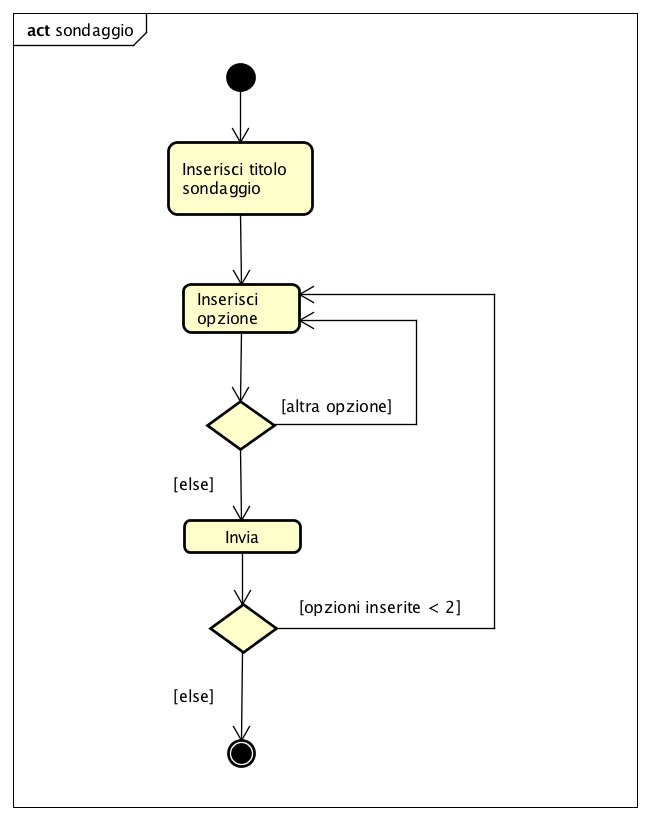
\includegraphics[scale=0.5]{img/Sondaggio.png}
  \captionof{figure}{Diagramma di attività per la bolla sondaggio} 
\end{center}




\subsection{configurazione ListBubble}
Questo diagramma rappresenta la configurazione della bolla ListBubble. Il flusso inizia con l’inserimento del titolo della lista. Dopo questo processo il flusso raggiunge il nodo decisione dove l’utente sceglie il modo di inserimento degli elementi. L’inserimento degli elementi avviene o manualmente (inserisci elemento manualmente) oppure con la selezione nella lista degli elementi predefiniti (inserisci elemento da checklist). Nel caso l’utente scegliesse di inserire un elemento dalla checklist predefinita, il flusso raggiunge il nodo decisione. Da questo punto l’utente può scegliere di inviare la bolla già configurata e il flusso raggiunge il nodo terminale, oppure scegliere di ritornare nel nodo decisione raggiunto precedentemente per poter inserire un altro elemento. Anche nel caso in cui l’utente scegliesse di inserire un elemento manualmente il flusso segue lo stesso percorso, ovvero l’utente inserisce l’elemento e decide di inviare la bolla con il raggiungendo il nodo terminale oppure inserire un altro elemento.

\begin{center}
  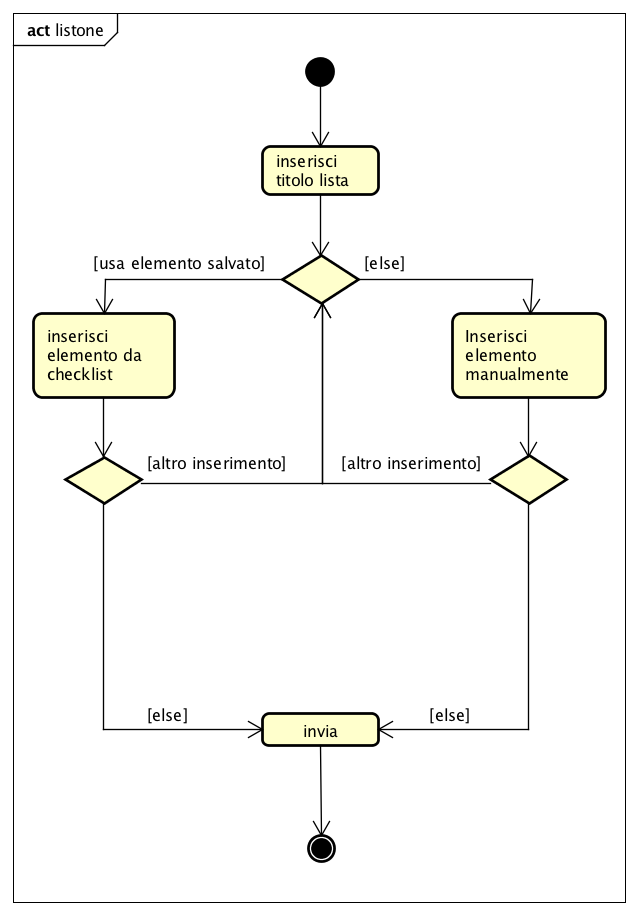
\includegraphics[scale=0.5]{img/ListBubble.png}
  \captionof{figure}{Diagramma di attività per la bolla ListBubble}
\end{center}



\section{Diagramma di Sequenza}



\section{Design Pattern}

\section{Tracciamento}




\appendix



\section{Descrizione Design Pattern}

Un design pattern è una soluzione progettuale elegante e generale ad un problema ricorrente. In particolare si tratta di una descrizione o modello logico da applicare per la risoluzione di un problema che può presentarsi in diverse situazioni durante la fase di progettazione e sviluppo del software, ancora prima della definizione dell'algoritmo ricorsivo della parte computazionale. Essi si suddividono in quattro categorie: \

\begin{itemize}
	\item \textbf{Architetturali :} esprimono schemi di base per impostare l'organizzazione strutturale di un sistema software;
	\item \textbf{Creazionali :} forniscono un'astrazione del processo di istanziazione degli oggetti;
	\item \textbf{Strutturali :} si occupano delle modalità di composizione di classi e oggetti per formare strutture complesse;
	\item \textbf{Comportamentali :} si occupano di algoritmi e dell'assegnamento di responsabilità tra oggetti collaboranti.

\end{itemize}

\subsection{Design Pattern Utilizzati}

\subsubsection{Factory Method}
Rappresenta uno dei pattern creazionali adottati dal gruppo Obelix, esso  indirizza il problema della creazione di oggetti senza specificarne l'esatta classe. Questo pattern raggiunge il suo scopo fornendo un'interfaccia per creare un oggetto, ma lascia che le sottoclassi decidano quale oggetto istanziare.

	\FloatBarrier
	\begin{figure}[ht]
		\centering
		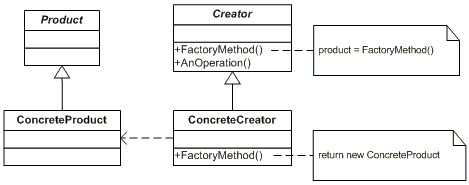
\includegraphics[scale=0.45]{img/method.jpg}
		\caption{factory method}
	\end{figure}


Product definisce l'interfaccia implementata da ConcreteProduct, creator definisce il factory method che restituisce una interfaccia di tipo product, ConcreteCreator definisce il metodo factory effettivo per la creazione di un’istanza particolare di tipo Product.


I motivi che portano alla scelta del suo utilizzo sono:

\begin{itemize}
\item La creazione di un oggetto preclude il suo riuso senza una significativa duplicazione di codice
\item  La creazione di un oggetto richiede l'accesso ad informazioni o risorse che non dovrebbero essere contenute nella classe di composizione
\item La gestione del ciclo di vita degli oggetti gestiti deve essere centralizzata in modo da assicurare un comportamento coerente all'interno dell'applicazione

\end{itemize}


polyglot.js
money.js
weather.js























